\section{Results}
\label{sec:results}

We first report the proxy check (RQ2), then the searches and the test comparison of the three arms (RQ1), and then the change from studio to real-world and Indian photographs (RQ3).

\subsection{Proxy Validity}
\label{subsec:res-proxy}

The proxy passed the check that was fixed before the \genone searches (Section~\ref{subsec:proxy}). The Spearman rank correlation between the proxy scores and the 40-epoch medium scores is $\rho = 0.976$ ($n = 8$), well above the threshold of 0.6 (Table~\ref{tab:proxy}, Fig.~\ref{fig:proxy}). The two rankings differ only in one swap of neighbors, lhs3 and lhs5. The same four settings are at the top of both rankings, with the defaults second behind lhs4 in both. Their medium scores, however, are within 0.026 of each other. The proxy is therefore good at telling poor settings from good ones and much less good at ordering the good ones.

\begin{table}[!t]
\centering
\caption{Proxy-Validity Check (\genone, Validation \mapfifty)}
\label{tab:proxy}
\footnotesize
\begin{tabular}{@{}lcccc@{}}
\toprule
Setting & Proxy & Rank & Medium & Rank \\
\midrule
lhs1 & 0.08687 & 1 & 0.28423 & 1 \\
lhs2 & 0.23077 & 2 & 0.49451 & 2 \\
lhs3 & 0.29495 & 3 & 0.56712 & 4 \\
lhs5 & 0.30186 & 4 & 0.55195 & 3 \\
lhs7 & 0.37560 & 5 & 0.61246 & 5 \\
lhs6 & 0.44285 & 6 & 0.62161 & 6 \\
Defaults & 0.47648 & 7 & 0.62884 & 7 \\
lhs4 & 0.49547 & 8 & 0.63839 & 8 \\
\midrule
\multicolumn{5}{@{}l@{}}{Spearman $\rho = 0.976$, $n = 8$; pass threshold $\rho \ge 0.6$} \\
\bottomrule
\end{tabular}
\\[2pt]
\parbox{\columnwidth}{\footnotesize Proxy: 12 epochs on the stratified 40\% training subset. Medium: 40 epochs on the full training split. Both at 416~px; rank 1 is the lowest score. lhs1--lhs7 are the Latin hypercube settings.}
\end{table}

\begin{figure}[!t]
\centering
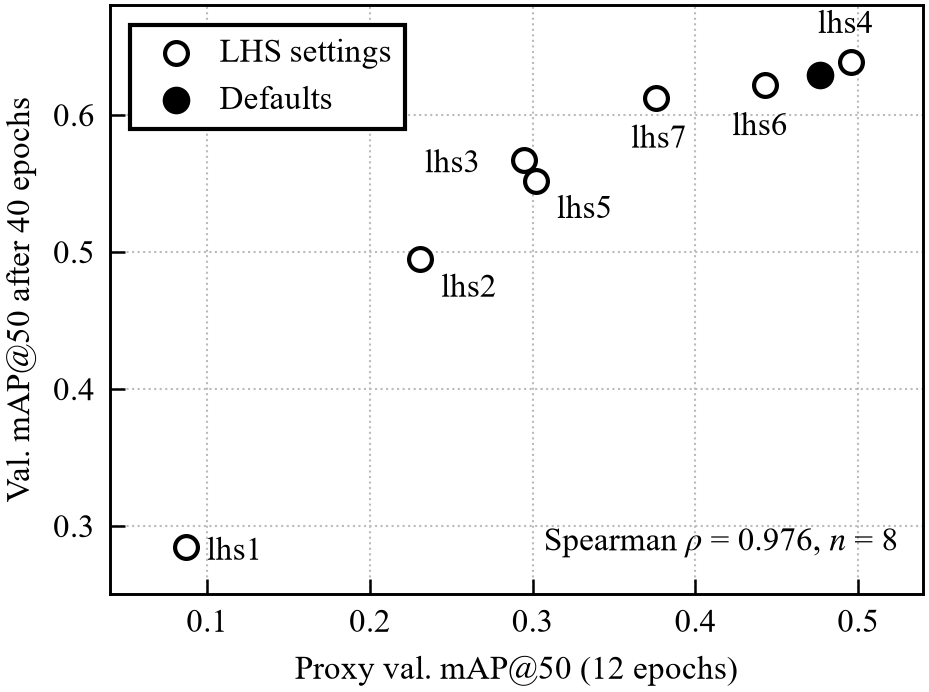
\includegraphics[width=\columnwidth]{r_proxy.png}
\caption{Proxy score against the 40-epoch (medium) validation \mapfifty for the eight settings of the \genone proxy check. The two rankings agree except for the neighbors lhs3 and lhs5.}
\label{fig:proxy}
\end{figure}

A second, indirect check comes from configurations that both generations evaluated. Since the seeds and the search space were the same, random search drew the same 32 configurations in both generations. PSO positions depend on the fitness only through the personal and global bests, and these coincided for long enough that the swarm visited identical positions in rounds 1 to 3 (24 evaluations), though not in round~4. On these repeated configurations the proxy scores of the two generations have Spearman correlations of 0.991 (random search) and 0.892 (PSO), computed from the four search logs. This compares proxy with proxy and not proxy with longer training. It shows that the two generations order settings in a similar way, but it does not replace a proxy check for \gentwo.

\subsection{Search Behavior}
\label{subsec:res-search}

Fig.~\ref{fig:convergence} shows every proxy evaluation and the best score so far. In \genone, random search found its best setting (0.4995 proxy \mapfifty) at its second evaluation and never improved on it. PSO improved in steps, from 0.4894 after round~1 to 0.4942 after round~3 and 0.4953 in round~4 (evaluation 27). The swarm converged as it should: the round means rose from 0.393 to 0.423, 0.450 and 0.482, and the standard deviation within a round fell from 0.122 to 0.088, 0.047 and 0.011. The defaults scored 0.4765 on the same proxy, which is higher than 28 of the 32 random-search evaluations and 21 of the 32 PSO evaluations. The two winners differ by only 0.0042, and lhs4 from the proxy check (0.4955) lies between them. All four search winners in the two generations use an initial learning rate below the default of 0.01 (0.0025 to 0.0070).

\begin{figure*}[!t]
\centering
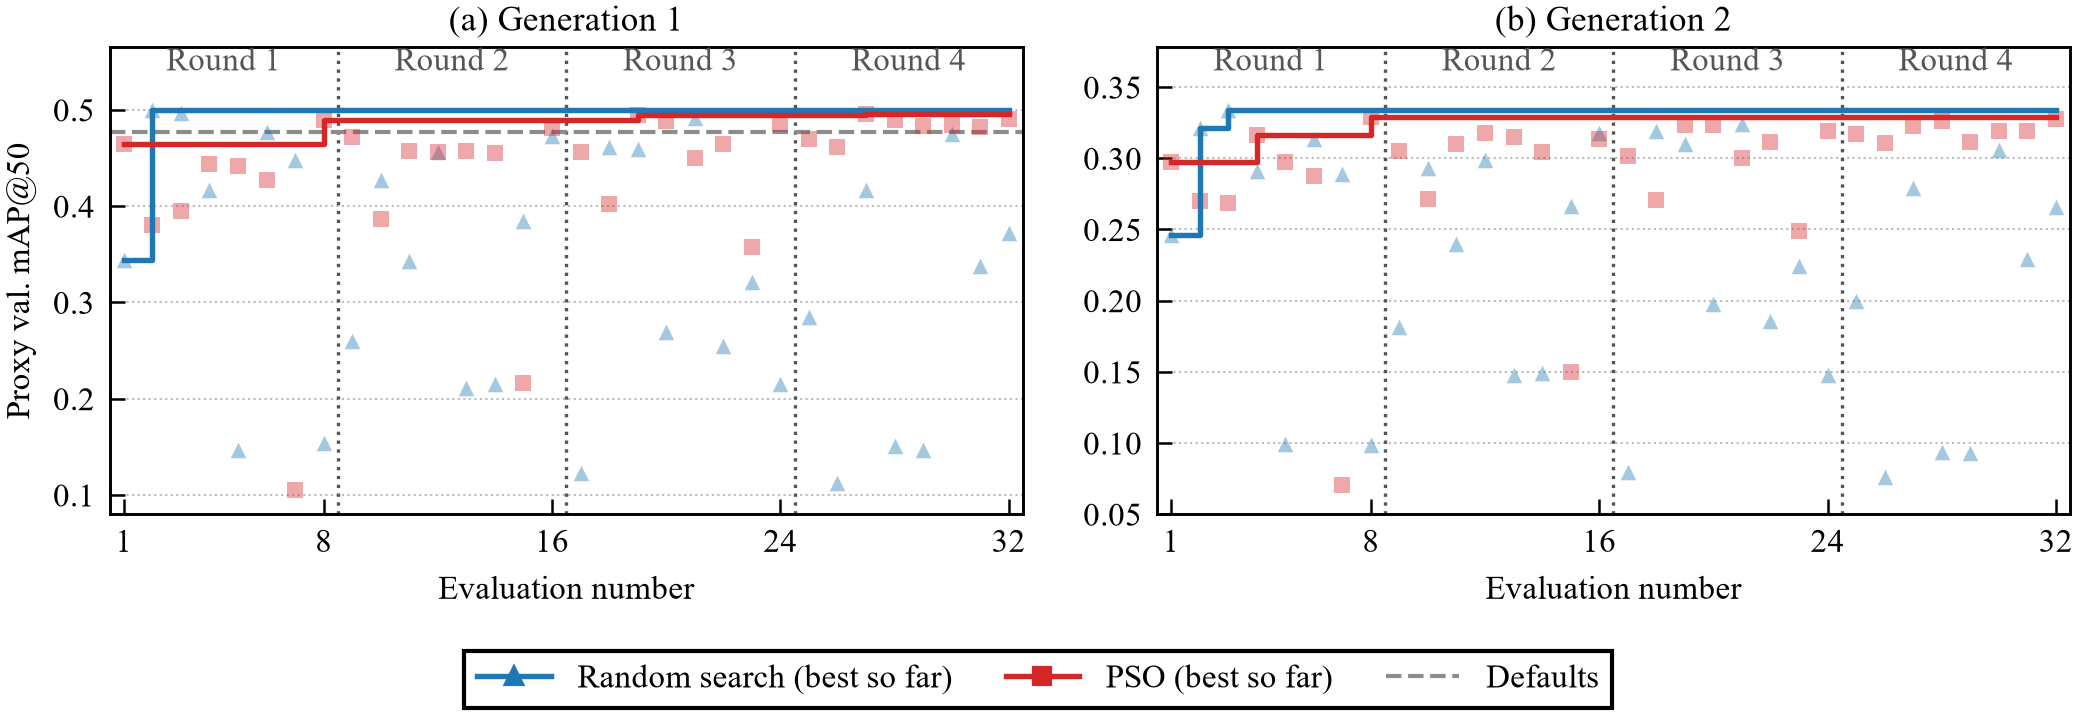
\includegraphics[width=\textwidth]{r_convergence.png}
\caption{Proxy scores during the searches. Faint markers are single evaluations (triangles: random search, squares: PSO) and the solid lines show the best score so far. Dotted vertical lines separate the four PSO rounds of eight particles. The dashed line in (a) is the proxy score of the defaults, which was not measured in \gentwo. The two panels use different validation sets, classes and image sizes, so their scores should not be compared.}
\label{fig:convergence}
\end{figure*}

In \gentwo, random search again peaked early (0.3340 at evaluation~3). The best PSO score, 0.3290, came from the last particle of round~1 and was never beaten; the best scores of the later rounds were 0.3176, 0.3237 and 0.3279. The swarm still converged, with round means rising from 0.267 to 0.286, 0.300 and 0.319 and the within-round standard deviation falling from 0.082 to 0.006. In both generations the mean proxy score over all 32 evaluations was higher for PSO than for random search (0.437 against 0.333 in \genone, 0.293 against 0.226 in \gentwo). The swarm spent its later evaluations near good points, which raises the mean, but it did not find better points. We have no \gentwo proxy run of the defaults, so we do not know where they would stand.

\subsection{Generation~1 Test Results (Studio Data)}
\label{subsec:res-gen1}

Table~\ref{tab:gen1-test} gives the test results of the three \genone models on the 1,046 studio test images. (The evaluator counts 7,415 boxes; Table~\ref{tab:datasets} lists 7,413 because it leaves out 2 zero-size boxes.) The arms score 0.676 (A), 0.672 (B) and 0.668 (C) \mapfifty, and every pairwise 95\% interval contains 0 on both metrics. The largest difference is C$-$A, $-0.008$ [$-0.021$, $+0.007$]. On studio data the three arms are statistically tied, and if anything the point estimates put the defaults first and PSO last. Precision and recall are almost identical. Validation gave a similar picture: the defaults and PSO both reached 0.657, while random search, whose setting had the highest proxy score in \genone, reached the lowest value, 0.643.

\begin{table*}[!t]
\centering
\caption{\genone Test Results on the Studio Test Split (1,046 Images)}
\label{tab:gen1-test}
\footnotesize
\begin{tabular}{@{}lcccccc@{}}
\toprule
Arm & Val \mapfifty & Test \mapfifty [95\% CI] & Test \mapfiftyninetyfive [95\% CI] & P & R & ms/img \\
\midrule
A: Defaults & 0.657 & 0.676 [0.639, 0.722] & 0.474 [0.441, 0.518] & 0.747 & 0.581 & 31.4 \\
B: Random search & 0.643 & 0.672 [0.634, 0.717] & 0.475 [0.441, 0.519] & 0.746 & 0.587 & 38.3 \\
C: PSO & 0.657 & 0.668 [0.627, 0.717] & 0.471 [0.437, 0.516] & 0.747 & 0.586 & 31.7 \\
\bottomrule
\end{tabular}
\\[6pt]
\begin{tabular}{@{}lccccc@{}}
\toprule
Pair & $\Delta$\mapfifty [95\% CI] & $P(\Delta>0)$ & $\Delta$\mapfiftyninetyfive [95\% CI] & $P(\Delta>0)$ & Verdict \\
\midrule
B$-$A & $-0.004$ [$-0.016$, $+0.009$] & 0.30 & $+0.001$ [$-0.008$, $+0.010$] & 0.59 & not significant \\
C$-$A & $-0.008$ [$-0.021$, $+0.007$] & 0.16 & $-0.003$ [$-0.012$, $+0.007$] & 0.34 & not significant \\
C$-$B & $-0.004$ [$-0.015$, $+0.007$] & 0.24 & $-0.003$ [$-0.011$, $+0.004$] & 0.19 & not significant \\
\bottomrule
\end{tabular}
\\[2pt]
\parbox{\textwidth}{\footnotesize Val: best checkpoint on the validation split after 100 epochs. CIs: 1,000 paired bootstrap resamples of the test images. P and R at the confidence of maximum F1. ms/img: median batch-1 latency at 416~px on a laptop CPU (Intel Core Ultra~5 125H). $P(\Delta>0)$: share of resamples in which the first arm of the pair scored higher. A difference is significant only if its CI excludes 0.}
\end{table*}

Per class (Fig.~\ref{fig:gen1-perclass}), the arms differ by less than 0.02 AP@50 on five of the six classes. The exception is PLASTIC, where PSO scores 0.638 against 0.699 (A) and 0.693 (B). PSO is highest on BIODEGRADABLE, GLASS and METAL. Per-class AP has no confidence interval (Section~\ref{subsec:eval}), so we do not read much into these differences. The three networks have the same architecture, so the higher CPU latency of B in Table~\ref{tab:gen1-test} most likely comes from other load on the laptop during timing.

\begin{figure}[!t]
\centering
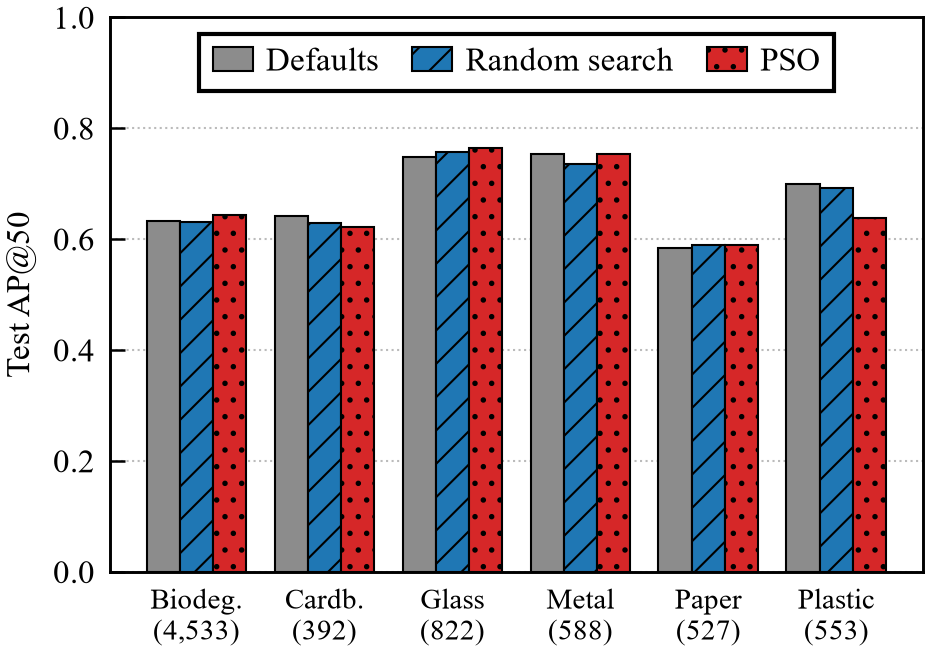
\includegraphics[width=\columnwidth]{r_gen1_per_class.png}
\caption{Per-class test AP@50 of the three \genone models on the studio test set. The number under each class is its number of test boxes as counted by the evaluator.}
\label{fig:gen1-perclass}
\end{figure}

\subsection{Generation~2 Test Results (Mixed Data)}
\label{subsec:res-gen2}

Table~\ref{tab:gen2-test} gives the \gentwo test results on the whole test split and on each domain. On the whole split the defaults score 0.479, random search 0.497 and PSO 0.500 \mapfifty. Both tuned arms are significantly better than the defaults (B$-$A $+0.017$ [$+0.006$, $+0.030$], C$-$A $+0.020$ [$+0.011$, $+0.032$]), but PSO and random search cannot be told apart (C$-$B $+0.003$ [$-0.008$, $+0.015$]). The intervals of the single arms overlap widely. The gains show up only in the paired differences, because the paired bootstrap removes the variation in image difficulty that all three models share. The \mapfiftyninetyfive verdicts agree with the \mapfifty verdicts everywhere. Random search was ahead of PSO on validation (0.473 against 0.466), but on test the two are tied.

Studio images account for 7,413 of the 8,192 boxes, and the studio test set alone (the 1,046 \genone test images) gives the same result: B$-$A ($+0.024$) and C$-$A ($+0.019$) are significant and C$-$B ($-0.005$) is not. PSO and random search differ significantly only on the Indian test set, where all scores are close to zero (Section~\ref{subsec:res-domain}).

\begin{table*}[!t]
\centering
\caption{\gentwo Test Results per Test Set: \mapfifty and \mapfiftyninetyfive [95\% CI] per Arm, and Pairwise Differences in \mapfifty}
\label{tab:gen2-test}
\footnotesize
\begin{tabular}{@{}lcccc@{}}
\toprule
 & All & Studio & Real-world & India (DWSD) \\
 & 1,514 img., 8,192 boxes & 1,046 img., 7,413 boxes & 468 img., 779 boxes & 700 img., 4,502 boxes \\
\midrule
\multicolumn{5}{@{}l}{\textit{Test \mapfifty [95\% CI]}} \\
A: Defaults & 0.479 [0.453, 0.513] & 0.571 [0.529, 0.619] & 0.310 [0.278, 0.440] & 0.027 [0.024, 0.031] \\
B: Random search & 0.497 [0.471, 0.531] & 0.595 [0.557, 0.639] & 0.298 [0.271, 0.407] & 0.023 [0.021, 0.027] \\
C: PSO & 0.500 [0.474, 0.534] & 0.590 [0.550, 0.635] & 0.310 [0.279, 0.415] & 0.027 [0.024, 0.031] \\
\midrule
\multicolumn{5}{@{}l}{\textit{$\Delta$\mapfifty [95\% CI] (bold: significant, CI excludes 0)}} \\
B$-$A & $\mathbf{+0.017}$ [$+0.006$, $+0.030$] & $\mathbf{+0.024}$ [$+0.009$, $+0.038$] & $-0.012$ [$-0.118$, $+0.053$] & $\mathbf{-0.003}$ [$-0.006$, $-0.001$] \\
C$-$A & $\mathbf{+0.020}$ [$+0.011$, $+0.032$] & $\mathbf{+0.019}$ [$+0.005$, $+0.033$] & $+0.001$ [$-0.111$, $+0.065$] & $+0.000$ [$-0.003$, $+0.003$] \\
C$-$B & $+0.003$ [$-0.008$, $+0.015$] & $-0.005$ [$-0.018$, $+0.009$] & $+0.013$ [$-0.015$, $+0.036$] & $\mathbf{+0.003}$ [$+0.001$, $+0.006$] \\
\midrule
\multicolumn{5}{@{}l}{\textit{Test \mapfiftyninetyfive [95\% CI]}} \\
A: Defaults & 0.329 [0.309, 0.358] & 0.386 [0.356, 0.425] & 0.254 [0.224, 0.371] & 0.015 [0.013, 0.018] \\
B: Random search & 0.342 [0.322, 0.372] & 0.404 [0.374, 0.442] & 0.238 [0.213, 0.330] & 0.013 [0.012, 0.015] \\
C: PSO & 0.343 [0.323, 0.374] & 0.398 [0.367, 0.439] & 0.248 [0.220, 0.336] & 0.015 [0.013, 0.017] \\
\bottomrule
\end{tabular}
\\[2pt]
\parbox{\textwidth}{\footnotesize All test sets were scored once, at 640~px, with 1,000 paired bootstrap resamples per test set. ``All'' is the whole \gentwo test split (studio plus real-world); India is DWSD, used for testing only. The \mapfiftyninetyfive differences give the same verdict as the \mapfifty differences in every cell. Validation \mapfifty: A 0.454, B 0.473, C 0.466.}
\end{table*}

Per class on the whole split, PSO has the highest AP@50 on five of the seven classes, random search on BIODEGRADABLE and PLASTIC, and the defaults on none. OTHER is very weak for every arm (AP@50 0.050 to 0.063); all 132 OTHER test boxes are in the real-world images. Precision rises from 0.549 (A) to 0.563 (B) and 0.582 (C), and recall from 0.445 (A) to 0.470 for both tuned arms. The median latency on the T4 at 640~px is 8.1 to 8.7~ms per image.

\subsection{Domain Gap}
\label{subsec:res-domain}

Averaged over the three \gentwo arms, test \mapfifty falls from about 0.59 on studio images to 0.31 on real-world images and 0.03 on Indian images (Fig.~\ref{fig:domains}). For every arm the real-world score is roughly half the studio score.

\begin{figure}[!t]
\centering
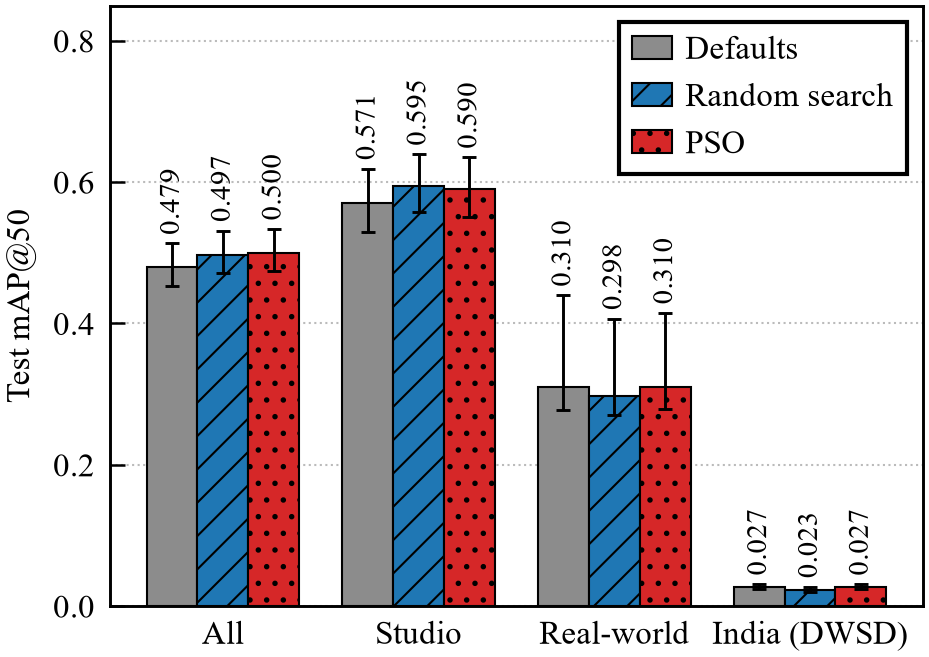
\includegraphics[width=\columnwidth]{r_domains.png}
\caption{Test \mapfifty of the three \gentwo models on each test set. Error bars are 95\% paired-bootstrap confidence intervals. ``All'' is the studio and real-world test images together. The real-world intervals are lopsided because that set has a single BIODEGRADABLE box.}
\label{fig:domains}
\end{figure}

On the 468 real-world test images (TACO and HITL), no pairwise difference is significant (Table~\ref{tab:gen2-test}). The intervals are wide and lopsided because BIODEGRADABLE has a single box in this set. Whether a resample leaves out or repeats that one image swings the AP of the class, which is one seventh of the mean, and the arms score 0.249 (A), 0.020 (B) and 0.003 (C) AP@50 on that box. The B$-$A and C$-$A intervals are 0.17 to 0.18 wide, so this test set cannot resolve differences of the size we measured on studio images (about 0.02).

On the 700 DWSD images from India all three models fail. They reach 0.023 to 0.027 \mapfifty, precision 0.070 to 0.075 and recall 0.043 to 0.047, and only PLASTIC (0.089 to 0.101) and PAPER (0.028 to 0.035) exceed 0.01 AP@50. The defaults and PSO are both significantly above random search and do not differ from each other. On \mapfiftyninetyfive the two significant differences are B$-$A $-0.002$ [$-0.003$, $-0.001$] and C$-$B $+0.002$ [$+0.000$, $+0.003$], where the lower bound is 0.0004 before rounding. These are differences of a few thousandths on scores near zero and have no practical meaning.

We know of four reasons for this failure (Section~\ref{subsec:datasets}). No Indian image was used for training, search or model selection. The DWSD images look augmented (rotated, with black corners and color tints), unlike any training image. The DWSD boxes come from mask regions, so touching items of one class merge into one large box; a detection of a single item overlaps such a box poorly and is counted as a miss even when it is correct. And the mapping from mask values to classes was inferred from the images, with six of the fifteen values uncertain. The India score therefore reflects the difference in labeling style as well as the quality of the models. Fig.~\ref{fig:samples} shows the three models on two studio, two real-world and two DWSD test images. The two real-world images contain eight objects each; every model finds at most three objects in the first and none in the second. On the DWSD images each model predicts at most one box, against 4 and 19 ground-truth boxes. On the first of them all three models box the region that the ground truth labels PAPER, but call it PLASTIC.

\begin{figure*}[p]
\centering
\includegraphics[width=0.85\textwidth]{r_samples.jpg}
\caption{Detections of the three \gentwo models on two studio, two real-world and two Indian (DWSD) test images, next to the ground truth. The images were not picked by hand: for each test set we shuffled the images with at least three ground-truth boxes (seed 0) and took the first two. All models saw the same images at 640~px with a confidence threshold of 0.25 and an NMS IoU of 0.7. The number in the corner of each panel is the number of boxes. The DWSD ground-truth boxes come from mask regions, so touching items of one class can share a box.}
\label{fig:samples}
\end{figure*}

Because the two generations differ in classes, image size and training data, Tables~\ref{tab:gen1-test} and~\ref{tab:gen2-test} cannot be compared with each other. Table~\ref{tab:g1g2} therefore scores all six final models on the same studio and real-world test images, restricted to the six shared classes (Section~\ref{subsec:eval}). On the real-world images every \gentwo arm is significantly better than every \genone arm: 0.338 to 0.353 \mapfifty against 0.038 to 0.096, about four to nine times as high. On the studio images it is the other way round, and every \genone arm is significantly better than every \gentwo arm, by 0.074 to 0.105. Within each generation no real-world difference is significant (for example \genone C$-$A $+0.048$ [$-0.020$, $+0.163$] and \gentwo C$-$B $+0.013$ [$-0.019$, $+0.042$]), and the studio verdicts match Tables~\ref{tab:gen1-test} and~\ref{tab:gen2-test}. The 0.096 of \genone C and its wide interval are largely due to the single real-world BIODEGRADABLE box, on which that model scores 0.332 AP@50. The \gentwo models score higher on real-world images here than in Table~\ref{tab:gen2-test} (0.353 against 0.310 for A) only because OTHER is left out of the mean. As a sanity check, \genone reproduces its own studio test result within 0.0004 \mapfifty.

\begin{table}[!t]
\centering
\caption{\genone versus \gentwo on the Same Test Images: Test \mapfifty [95\% CI] on the Six Shared Classes}
\label{tab:g1g2}
\footnotesize
\begin{tabular}{@{}lcc@{}}
\toprule
Model (px) & Real-world (468 img.) & Studio (1,046 img.) \\
\midrule
G1 A (416) & 0.047 [0.038, 0.080] & 0.676 [0.641, 0.719] \\
G1 B (416) & 0.038 [0.031, 0.069] & 0.672 [0.636, 0.716] \\
G1 C (416) & 0.096 [0.041, 0.214] & 0.669 [0.628, 0.716] \\
\midrule
G2 A (640) & 0.353 [0.315, 0.504] & 0.571 [0.529, 0.619] \\
G2 B (640) & 0.338 [0.304, 0.473] & 0.595 [0.557, 0.639] \\
G2 C (640) & 0.352 [0.315, 0.485] & 0.590 [0.550, 0.635] \\
\midrule
$\Delta$ G2$-$G1 & $+0.243$ to $+0.315$ & $-0.105$ to $-0.074$ \\
\bottomrule
\end{tabular}
\\[2pt]
\parbox{\columnwidth}{\footnotesize G1, G2: \genone, \gentwo; each model was scored once at its own training image size (px). Real-world: 647 boxes after removing OTHER, with a single BIODEGRADABLE box; studio: 7,413 boxes, no OTHER. CIs: 1,000 paired bootstrap resamples per test set. $\Delta$: range over all nine G2$-$G1 pairs, every one significant; e.g., real-world G2 B$-$G1 C $+0.243$ [$+0.134$, $+0.418$], studio G2 A$-$G1 A $-0.105$ [$-0.125$, $-0.084$]. On the five real-world classes with more than one box, \gentwo scores 0.239--0.618 AP@50 and \genone 0.008--0.117.}
\end{table}

We also looked at where the \gentwo models do succeed on real-world photographs. For each of the 468 real-world test images we counted the image as fully correct if every ground-truth object is matched by a detection of the same class with IoU $\geq 0.5$ and no detection is left unmatched (greedy matching, highest confidence first, confidence threshold 0.25). The models are fully correct on 166 (A), 168 (B) and 170 (C) images, 35 to 36\% of the set, and all three are correct on the same 111. Nearly all of these are single-object photographs. Of the 375 images with one object, the models get 164 to 167 fully right; of the 47 with two objects, 1 to 4; and of the 46 with three or more, none. Fig.~\ref{fig:best} shows the best cases. No image with three or more objects is fully correct for all three models and only one image with two objects is, so for the figure we took the two images with at least two objects that at least two models get fully right. One of them is a close-up on a plain background, which is close to studio conditions. In short, the models can handle a single item in a real scene but not a cluttered scene with several items.

\begin{figure*}[!t]
\centering
\includegraphics[width=0.8\textwidth]{r_best.jpg}
\caption{Success cases on real-world test images. These are favorable examples and are not typical. Rows 1 and 2 are the only real-world test images with two or more objects that at least two of the three \gentwo models get fully right (every object found with the right class and no false detection); random search (B) misses one object in row 1. Rows 3 and 4 are the first two, in a seed-0 shuffle, of the 110 single-object images that all three models get fully right. Settings as in Fig.~\ref{fig:samples}.}
\label{fig:best}
\end{figure*}

\subsection{Compute Cost}
\label{subsec:res-cost}

Table~\ref{tab:compute} lists the recorded GPU time of every run on one Tesla T4. It covers training only; setup, data copies and idle time are excluded. Counting its search, each tuned arm cost about 2.7 to 2.8 times the GPU time of Arm~A. The budget was equal in evaluations and not in time: the mean proxy training took 214.3~s for PSO and 238.7~s for random search in \genone, and 285.5~s and 259.0~s in \gentwo. The largest item in \genone was the proxy check, in which the eight 40-epoch medium runs took 3.84 of 4.36 hours. In \gentwo about 24 more GPU-hours were lost when two sessions froze and sat idle until the 12-hour limit of the platform; these hours are not in the totals. The test evaluation took 283.1~s on the laptop CPU in \genone and 220.6~s on the T4 for the four \gentwo test sets.

\begin{table}[!t]
\centering
\caption{Recorded GPU Time per Run (Hours, One Tesla T4)}
\label{tab:compute}
\footnotesize
\begin{tabular}{@{}lcc@{}}
\toprule
Run & \genone & \gentwo \\
\midrule
Proxy-validity check (16 runs) & 4.36 & not run \\
PSO search (32 proxy trainings) & 1.91 & 2.54 \\
Random search (32 proxy trainings) & 2.12 & 2.30 \\
Arm~A full training (100 epochs) & 1.18 & 1.56 \\
Arm~B full training (100 epochs) & 1.15 & 2.07 \\
Arm~C full training (100 epochs) & 1.45 & 1.60 \\
\midrule
Total recorded & 12.18 & 10.06 \\
\bottomrule
\end{tabular}
\\[2pt]
\parbox{\columnwidth}{\footnotesize Sums of the recorded training wall-clock times. The \gentwo random search and Arm~C training were resumed after a session froze (Arm~C after epoch 55); their idle time, about 24 GPU-hours in total, is not included.}
\end{table}
